\documentclass[11pt]{article}
\usepackage[utf8]{inputenc}
\usepackage[T1]{fontenc}
\usepackage[a4paper,margin=2.2cm,top=2.6cm]{geometry}
\usepackage{amsmath,amssymb}
\usepackage{graphicx}
\usepackage{enumitem}
\usepackage{xcolor}
\usepackage[most]{tcolorbox}
\usepackage{fancyhdr}
\usepackage[some]{background}
\usepackage{icomma}
\usepackage{tikz}
\usetikzlibrary{calc}

\definecolor{navy}{RGB}{20,40,75}
\definecolor{itsblue}{RGB}{18,86,130}
\definecolor{gold}{RGB}{233,170,40}
\definecolor{soalblue}{RGB}{31,78,121}
\definecolor{pembgreen}{RGB}{30,120,80}
\definecolor{boxbg}{RGB}{233,240,250}

\pagestyle{fancy}\fancyhf{}
\lhead{\small\scshape Matematika}
\chead{\small www.tiktok.com/@result\_han}
\rhead{\small\scshape @result\_han}
\cfoot{\small Halaman \thepage}
\renewcommand{\headrulewidth}{0.4pt}

\backgroundsetup{scale=6,color=black!7,opacity=0.7,angle=45,
  position=current page.center,contents={@result\_han}}

% kotak soal: #1 = topik (boleh kosong), #2 = nomor
\newtcolorbox{soalbox}[2][]{breakable,colback=boxbg,colframe=soalblue,
  coltitle=white,fonttitle=\bfseries\sffamily,
  title={\mbox{Nomor #2}\hfill{\normalfont\itshape\small #1}},
  boxrule=0.8pt,arc=3pt,left=3mm,right=3mm,top=2mm,bottom=2mm}
\newtcolorbox{pembox}{breakable,colback=pembgreen!6,colframe=pembgreen,
  coltitle=white,fonttitle=\bfseries\sffamily,title=Pembahasan,
  boxrule=0.8pt,arc=3pt,left=3mm,right=3mm,top=2mm,bottom=2mm}
\newtcolorbox{catatanbox}{colback=gold!10,colframe=gold!85!black,
  coltitle=black,fonttitle=\bfseries\sffamily,title=Catatan redaksi,
  boxrule=0.7pt,arc=2pt,left=3mm,right=3mm,top=1.2mm,bottom=1.2mm}

\newenvironment{pil}{\begin{enumerate}[label=(\Alph*),leftmargin=*,itemsep=1pt,topsep=3pt]}{\end{enumerate}}
\newcommand{\jw}[1]{\par\smallskip\noindent\colorbox{gold!18}{\parbox{0.97\textwidth}{\textbf{Jawaban:} #1}}}
\newcommand{\fig}[1]{\begin{center}#1\end{center}}

% pembatas bagian dengan mini-sampul
\newcommand{\bagian}[4]{\clearpage\thispagestyle{empty}%
\noindent
\begin{tikzpicture}\fill[itsblue](0,0)rectangle(\textwidth,-1.5);
\fill[gold](0,-1.5)rectangle(\textwidth,-1.62);
\node[anchor=north,text=white,font=\sffamily\bfseries\large]at(0.5\textwidth,-0.45){Latihan Seleksi Mandiri ITS};
\end{tikzpicture}
\vspace{1.3cm}
\begin{center}
\includegraphics[height=1.9cm]{images/7/7-1.png}\hspace{1.2cm}\raisebox{0.3cm}{\includegraphics[height=1.3cm]{#3}}\\[1.3em]
{\Huge\bfseries Matematika}\\[0.4em]
{\LARGE #1}\\[0.5em]
{\large #2}\\[1.1em]
\fbox{\parbox{0.74\textwidth}{\centering
Pengetikan ulang dan pemformatan: \textbf{@result\_han}\\[0.2em]
Follow TikTok: \textbf{www.tiktok.com/@result\_han}\\[0.2em]
Paket soal PTN lainnya: \textbf{lynk.id/result\_han}}}\\[1em]
{\small\itshape #4}
\end{center}
\clearpage}

\linespread{1.04}
\begin{document}

%================= SAMPUL UTAMA =================
\thispagestyle{empty}
\noindent\begin{tikzpicture}\fill[navy](0,0)rectangle(\textwidth,-3.2);
\fill[itsblue!25](\textwidth-2,0)circle(1.6);
\node[anchor=north west,text=white,font=\sffamily\bfseries\large]at(0.4,-0.5){INSTITUT TEKNOLOGI SEPULUH NOPEMBER};
\node[anchor=north west,text=white!80,font=\sffamily\small]at(0.4,-1.05){Seleksi Mandiri 2024};
\node[anchor=north west,text=gold,font=\sffamily\bfseries]at(0.4,-1.5){BIDANG MATEMATIKA};
\node[anchor=north west]at(0.4,-0.4){\includegraphics[height=1.4cm]{images/7/7-1.png}};
\end{tikzpicture}
\vspace{1.2cm}
\begin{center}
{\Huge\bfseries SOAL ASLI}\\[0.3em]
{\Huge\bfseries SELEKSI MANDIRI ITS 2024}\\[0.5em]
{\large Rekonstruksi Soal, Jawaban, dan Pembahasan}\\[1.6em]
\includegraphics[width=0.30\textwidth]{images/7/7-2.png}\\[0.4em]
{\small\itshape Cuplikan tampilan soal asli SM ITS 2024.}\\[1.4em]
\fbox{\parbox{0.8\textwidth}{\centering
Dokumen ini disusun sebagai bahan belajar matematika untuk persiapan Seleksi Mandiri ITS. Penyajian dibuat ulang dengan format LaTeX yang rapi serta pembahasan setelah setiap soal.\\[0.4em]
Formatting dan pengetikan ulang oleh \textbf{@result\_han}}}
\end{center}
\vfill
\begin{center}\small Berisi 4 bagian: Soal Asli SM ITS 2024 serta Set Soal 1, 2, dan 3.\end{center}

%==================================================================
%  BAGIAN I : SOAL ASLI SM ITS 2024 (22 SOAL, A--D)
%==================================================================
\bagian{Soal Asli SM ITS 2024}{22 Soal Pilihan Ganda dan Pembahasan}{images/7/7-1.png}{Format Soal -- Jawaban -- Pembahasan.}

{\noindent\Large\bfseries Bagian I\quad Soal Asli SM ITS 2024\par}\smallskip
{\noindent\small Setiap nomor disusun dalam format soal, pembahasan, dan pilihan yang benar.\par}\medskip\hrule\medskip

\begin{soalbox}[Matriks]{1}
Diketahui $\begin{pmatrix}2&1\\1&3\end{pmatrix}\begin{pmatrix}x&2\\1&y\end{pmatrix}=\begin{pmatrix}7&10\\5&20\end{pmatrix}$. Nilai $x-y$ adalah \ldots
\begin{pil}\item $-4$ \item $-3$ \item $3$ \item $4$\end{pil}
\end{soalbox}
\begin{pembox}
Kalikan kedua matriks pada ruas kiri: $\begin{pmatrix}2x+1&4+y\\x+3&2+3y\end{pmatrix}$. Dengan menyamakan elemen yang bersesuaian, $2x+1=7\Rightarrow x=3$ dan $4+y=10\Rightarrow y=6$. Maka $x-y=3-6=-3$.
\jw{(B) $-3$}
\end{pembox}

\begin{soalbox}[Logaritma]{2}
Jika ${}^2\log 3=p$ dan ${}^2\log 5=q$, maka nilai ${}^6\log 45$ adalah \ldots
\begin{pil}\item $\dfrac{2p+q}{1+p}$ \item $\dfrac{p+2q}{1+p}$ \item $\dfrac{1+2p}{p+q}$ \item $\dfrac{2+p+q}{1+q}$\end{pil}
\end{soalbox}
\begin{pembox}
Gunakan perubahan basis ke basis 2: ${}^6\log 45=\dfrac{{}^2\log 45}{{}^2\log 6}$. Karena $45=3^2\cdot5$ dan $6=2\cdot3$, maka ${}^2\log45=2{}^2\log3+{}^2\log5=2p+q$ dan ${}^2\log6=1+p$. Jadi ${}^6\log45=\dfrac{2p+q}{1+p}$.
\jw{(A) $\dfrac{2p+q}{1+p}$}
\end{pembox}

\begin{soalbox}[Integral Substitusi]{3}
Hasil dari $\displaystyle\int\dfrac{6x-4}{\sqrt{3x^2-4x+7}}\,dx$ adalah \ldots
\begin{pil}\item $2\sqrt{3x^2-4x+7}+C$ \item $\sqrt{3x^2-4x+7}+C$ \item $\tfrac{1}{2}\sqrt{3x^2-4x+7}+C$ \item $\tfrac{2}{3}\sqrt{3x^2-4x+7}+C$\end{pil}
\end{soalbox}
\begin{pembox}
Misalkan $u=3x^2-4x+7$, maka $du=(6x-4)\,dx$. Integral menjadi $\int u^{-1/2}\,du=2u^{1/2}+C=2\sqrt{3x^2-4x+7}+C$.
\jw{(A) $2\sqrt{3x^2-4x+7}+C$}
\end{pembox}

\begin{soalbox}[Geometri Ruang]{4}
Sebuah balok berukuran panjang 10 cm, lebar 6 cm, dan tinggi 4 cm. Seekor semut bergerak dari salah satu titik sudut balok ke titik sudut yang berhadapan melalui permukaan balok. Jarak terpendek yang dapat ditempuh semut adalah \ldots
\fig{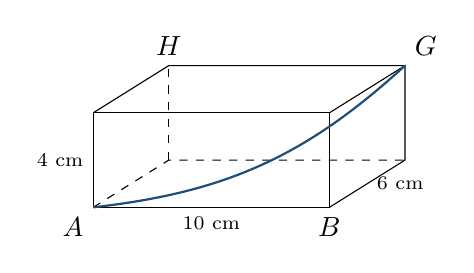
\begin{tikzpicture}[scale=0.6]
\coordinate(A)at(0,0);\coordinate(B)at(5,0);\coordinate(Bt)at(5,2);\coordinate(At)at(0,2);
\coordinate(Bb)at(6.6,1);\coordinate(Cb)at(6.6,3);\coordinate(Db)at(1.6,3);\coordinate(Ab)at(1.6,1);
\draw(A)--(B)--(Bt)--(At)--cycle;
\draw(B)--(Bb)--(Cb)--(Bt);\draw(At)--(Db)--(Cb);\draw[dashed](A)--(Ab)--(Bb);\draw[dashed](Ab)--(Db);
\draw[soalblue,thick](A)to[bend right=18](Cb);
\node[below left]at(A){$A$};\node[below]at(B){$B$};\node[above]at(Db){$H$};\node[above right]at(Cb){$G$};
\node[left]at($(A)!0.5!(At)$){\scriptsize 4 cm};\node[below]at($(A)!0.5!(B)$){\scriptsize 10 cm};\node[right]at($(B)!0.5!(Bb)$){\scriptsize 6 cm};
\end{tikzpicture}}
\begin{pil}\item $4\sqrt{17}$ cm \item $10\sqrt{2}$ cm \item $2\sqrt{58}$ cm \item $8\sqrt{5}$ cm\end{pil}
\end{soalbox}
\begin{pembox}
Lintasan terpendek pada permukaan balok diperoleh dengan membuka dua bidang menjadi satu bidang datar. Untuk dua titik sudut berhadapan, tiga kemungkinan jarak terpendek adalah
\[\sqrt{(10+6)^2+4^2}=\sqrt{272}=4\sqrt{17},\quad \sqrt{(10+4)^2+6^2}=\sqrt{232}=2\sqrt{58},\quad \sqrt{(6+4)^2+10^2}=\sqrt{200}=10\sqrt{2}.\]
Karena $10\sqrt2\approx14{,}14$ adalah yang terkecil, jarak terpendek adalah $10\sqrt2$ cm.
\jw{(B) $10\sqrt{2}$ cm}
\end{pembox}

\begin{soalbox}[Turunan Fungsi]{5}
Diketahui $f(x)=ax^2+bx-1$ dan $g(x)=bx^2+ax+2$. Jika $f'(2)=6$ dan $g'(-2)=-7$, maka nilai $3a-2b$ adalah \ldots
\begin{pil}\item $-3$ \item $-1$ \item $1$ \item $3$\end{pil}
\end{soalbox}
\begin{pembox}
$f'(x)=2ax+b$ dan $g'(x)=2bx+a$. Dari $f'(2)=6$: $4a+b=6$. Dari $g'(-2)=-7$: $-4b+a=-7$. Dari persamaan pertama $b=6-4a$; substitusi: $a-4(6-4a)=-7\Rightarrow 17a=17\Rightarrow a=1$, sehingga $b=2$. Maka $3a-2b=3-4=-1$.
\jw{(B) $-1$}
\end{pembox}

\begin{soalbox}[Limit Fungsi]{6}
Diketahui $\displaystyle\lim_{x\to c}(f(x)-g(x))=4$ dan $\displaystyle\lim_{x\to c}f(x)g(x)=5$. Nilai $\displaystyle\lim_{x\to c}(f(x)^2+g(x)^2)$ adalah \ldots
\begin{pil}\item $16$ \item $21$ \item $26$ \item $36$\end{pil}
\end{soalbox}
\begin{pembox}
Gunakan identitas $f^2+g^2=(f-g)^2+2fg$. Dengan sifat limit, $\lim(f^2+g^2)=4^2+2(5)=16+10=26$.
\jw{(C) $26$}
\end{pembox}

\begin{soalbox}[Vektor]{7}
Diketahui vektor $\vec a=(k,2,0)$ dan $\vec b=(1,0,0)$. Jika $k>0$ dan sudut antara $\vec a$ dan $\vec b$ adalah $60^\circ$, maka nilai $k$ adalah \ldots
\begin{pil}\item $\dfrac{\sqrt3}{3}$ \item $\dfrac{2\sqrt3}{3}$ \item $\sqrt3$ \item $2\sqrt3$\end{pil}
\end{soalbox}
\begin{pembox}
$\cos\theta=\dfrac{\vec a\cdot\vec b}{|\vec a||\vec b|}$. Di sini $\vec a\cdot\vec b=k$, $|\vec a|=\sqrt{k^2+4}$, $|\vec b|=1$. Maka $\dfrac{k}{\sqrt{k^2+4}}=\cos60^\circ=\tfrac12$. Kuadratkan: $\dfrac{k^2}{k^2+4}=\tfrac14\Rightarrow 4k^2=k^2+4\Rightarrow k^2=\tfrac43$. Karena $k>0$, $k=\dfrac{2}{\sqrt3}=\dfrac{2\sqrt3}{3}$.
\jw{(B) $\dfrac{2\sqrt3}{3}$}
\end{pembox}

\begin{soalbox}[Pertidaksamaan Linear]{8}
Nilai $x$ yang memenuhi pertidaksamaan $2(3x-1)-5\le x+8$ adalah \ldots
\begin{pil}\item $x\le3$ \item $x\ge3$ \item $x<-3$ \item $x>-3$\end{pil}
\end{soalbox}
\begin{pembox}
Sederhanakan ruas kiri: $2(3x-1)-5=6x-7$. Maka $6x-7\le x+8\Rightarrow 5x\le15\Rightarrow x\le3$.
\jw{(A) $x\le3$}
\end{pembox}

\begin{soalbox}[Komposisi Fungsi]{9}
Jika $f(x)=x^2-4x+1$ dan $g(x)=2x-3$, maka $f(g(x))$ adalah \ldots
\begin{pil}\item $4x^2-20x+22$ \item $4x^2-12x+10$ \item $2x^2-20x+22$ \item $4x^2+20x+22$\end{pil}
\end{soalbox}
\begin{pembox}
$f(g(x))=(2x-3)^2-4(2x-3)+1=(4x^2-12x+9)+(-8x+12)+1=4x^2-20x+22$.
\jw{(A) $4x^2-20x+22$}
\end{pembox}

\begin{soalbox}[Definisi Turunan]{10}
Jika $f(x)=3x^3-5x^2+7x-1$, maka $\displaystyle\lim_{h\to0}\dfrac{f(x+h)-f(x)}{h}$ adalah \ldots
\begin{pil}\item $9x^2-10x+7$ \item $3x^2-5x+7$ \item $9x^2+10x+7$ \item $x^2-10x+7$\end{pil}
\end{soalbox}
\begin{pembox}
Bentuk limit yang diberikan adalah definisi turunan $f'(x)$. Maka $f'(x)=9x^2-10x+7$.
\jw{(A) $9x^2-10x+7$}
\end{pembox}

\begin{soalbox}[Fungsi Implisit]{11}
Diketahui $f(3x-2)=2x^2+x+5$. Nilai $f(4)$ adalah \ldots
\begin{pil}\item $13$ \item $15$ \item $17$ \item $19$\end{pil}
\end{soalbox}
\begin{pembox}
Agar diperoleh $f(4)$, bagian dalam fungsi harus 4: $3x-2=4\Rightarrow x=2$. Substitusi: $f(4)=2(2)^2+2+5=15$.
\jw{(B) $15$}
\end{pembox}

\begin{soalbox}[Operasi Pecahan]{12}
Hitunglah $\dfrac34\div\dfrac98\times\dfrac25=\ldots$
\begin{pil}\item $\dfrac{4}{15}$ \item $\dfrac{5}{12}$ \item $\dfrac{2}{15}$ \item $\dfrac{8}{45}$\end{pil}
\end{soalbox}
\begin{pembox}
$\dfrac34\div\dfrac98=\dfrac34\times\dfrac89=\dfrac{24}{36}=\dfrac23$. Maka $\dfrac23\times\dfrac25=\dfrac{4}{15}$.
\jw{(A) $\dfrac{4}{15}$}
\end{pembox}

\begin{soalbox}[Limit Bentuk Tak Tentu]{13}
Nilai $\displaystyle\lim_{x\to9}\dfrac{x-9}{\sqrt{x}-3}$ adalah \ldots
\begin{pil}\item $3$ \item $6$ \item $9$ \item $12$\end{pil}
\end{soalbox}
\begin{pembox}
Substitusi langsung memberi $0/0$, sehingga kalikan dengan sekawan: $\dfrac{x-9}{\sqrt x-3}\cdot\dfrac{\sqrt x+3}{\sqrt x+3}=\sqrt x+3$. Maka limitnya $\sqrt9+3=6$.
\jw{(B) $6$}
\end{pembox}

\begin{soalbox}[Aljabar Dasar]{14}
Hasil pengembangan dari $(x-4)(x+7)$ adalah \ldots
\begin{pil}\item $x^2+3x-28$ \item $x^2-3x-28$ \item $x^2+11x-28$ \item $x^2-11x+28$\end{pil}
\end{soalbox}
\begin{pembox}
$(x-4)(x+7)=x^2+7x-4x-28=x^2+3x-28$.
\jw{(A) $x^2+3x-28$}
\end{pembox}

\begin{soalbox}[Luas Daerah]{15}
Luas daerah yang dibatasi oleh kurva $y=x^3$ dan $y=x$ adalah \ldots
\fig{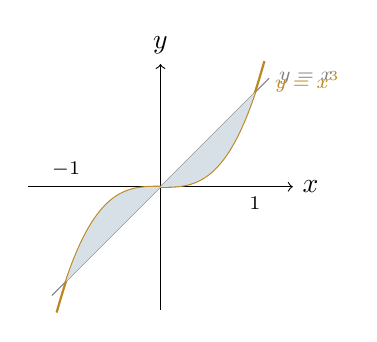
\begin{tikzpicture}[scale=1.2]
\draw[->](-1.4,0)--(1.4,0)node[right]{$x$};\draw[->](0,-1.3)--(0,1.3)node[above]{$y$};
\draw[domain=-1.15:1.15,smooth,variable=\x,gray] plot(\x,\x)node[right]{\scriptsize$y=x$};
\draw[domain=-1.1:1.1,smooth,variable=\x,gold!80!black,thick] plot(\x,{\x*\x*\x})node[below right]{\scriptsize$y=x^3$};
\fill[soalblue!18,domain=0:1,smooth,variable=\x] plot(\x,\x)--plot[domain=1:0](\x,{\x*\x*\x})--cycle;
\fill[soalblue!18,domain=-1:0,smooth,variable=\x] plot(\x,{\x*\x*\x})--plot[domain=0:-1](\x,\x)--cycle;
\node[below]at(1,0){\scriptsize$1$};\node[above]at(-1,0){\scriptsize$-1$};
\end{tikzpicture}}
\begin{pil}\item $\dfrac14$ \item $\dfrac13$ \item $\dfrac12$ \item $1$\end{pil}
\end{soalbox}
\begin{pembox}
Titik potong: $x^3=x\Rightarrow x(x^2-1)=0\Rightarrow x=-1,0,1$. Pada $0\le x\le1$, $y=x$ di atas $y=x^3$. Karena daerahnya simetris terhadap titik asal, luas total $=2\displaystyle\int_0^1(x-x^3)\,dx=2\left[\dfrac{x^2}{2}-\dfrac{x^4}{4}\right]_0^1=2\left(\dfrac12-\dfrac14\right)=\dfrac12$.
\jw{(C) $\dfrac12$}
\end{pembox}

\begin{soalbox}[Pertidaksamaan Nilai Mutlak]{16}
Himpunan penyelesaian dari $|2x-3|<5$ adalah \ldots
\begin{pil}\item $-1<x<4$ \item $x<-1$ atau $x>4$ \item $-4<x<1$ \item $x\le-1$ atau $x\ge4$\end{pil}
\end{soalbox}
\begin{pembox}
Untuk $|A|<b$ dengan $b>0$ berlaku $-b<A<b$. Maka $-5<2x-3<5\Rightarrow -2<2x<8\Rightarrow -1<x<4$.
\jw{(A) $-1<x<4$}
\end{pembox}

\begin{soalbox}[Operasi Pecahan]{17}
Hitunglah $\dfrac12+\dfrac23-\dfrac34+\dfrac16=\ldots$
\begin{pil}\item $\dfrac{5}{12}$ \item $\dfrac{7}{12}$ \item $\dfrac34$ \item $\dfrac{11}{12}$\end{pil}
\end{soalbox}
\begin{pembox}
Samakan penyebut menjadi 12: $\dfrac{6}{12}+\dfrac{8}{12}-\dfrac{9}{12}+\dfrac{2}{12}=\dfrac{6+8-9+2}{12}=\dfrac{7}{12}$.
\jw{(B) $\dfrac{7}{12}$}
\end{pembox}

\begin{soalbox}[Aritmetika]{18}
Tiga per delapan dari 1440 adalah \ldots
\begin{pil}\item $480$ \item $520$ \item $540$ \item $560$\end{pil}
\end{soalbox}
\begin{pembox}
$\dfrac38\times1440$: karena $1440\div8=180$, maka $\dfrac38\times1440=3\times180=540$.
\jw{(C) $540$}
\end{pembox}

\begin{soalbox}[Barisan Logaritma]{19}
Diketahui barisan $\ln3,\ \ln9,\ \ln27,\ \ln81,\ \ldots$. Jumlah delapan suku pertama barisan tersebut adalah \ldots
\begin{pil}\item $28\ln3$ \item $32\ln3$ \item $36\ln3$ \item $40\ln3$\end{pil}
\end{soalbox}
\begin{pembox}
Setiap suku $\ln3,\ln3^2,\ln3^3,\ldots$ dengan sifat $\ln(a^n)=n\ln a$ menjadi $\ln3,2\ln3,3\ln3,\ldots$ Jadi $U_n=n\ln3$ dan $S_8=(1+2+\cdots+8)\ln3=36\ln3$.
\jw{(C) $36\ln3$}
\end{pembox}

\begin{soalbox}[Deret Aritmetika]{20}
Jumlah dua belas bilangan kelipatan 4 pertama adalah \ldots
\begin{pil}\item $288$ \item $300$ \item $312$ \item $336$\end{pil}
\end{soalbox}
\begin{pembox}
Bilangannya $4,8,12,\ldots,48$, deret aritmetika $a=4$, $d=4$, $n=12$. $U_{12}=48$ dan $S_{12}=\dfrac{12}{2}(4+48)=6(52)=312$.
\jw{(C) $312$}
\end{pembox}

\begin{soalbox}[Eksponen]{21}
Bentuk sederhana dari $\dfrac{8x^3y^{-2}z^5}{24x^{-1}y^4z^{-3}}$ adalah \ldots
\begin{pil}\item $\dfrac13x^4y^{-6}z^8$ \item $\dfrac13x^2y^2z^2$ \item $3x^4y^{-6}z^8$ \item $\dfrac13x^{-4}y^6z^{-8}$\end{pil}
\end{soalbox}
\begin{pembox}
$\dfrac{8}{24}=\dfrac13$. Dengan $\dfrac{x^m}{x^n}=x^{m-n}$: $\dfrac{x^3}{x^{-1}}=x^4$, $\dfrac{y^{-2}}{y^4}=y^{-6}$, $\dfrac{z^5}{z^{-3}}=z^8$. Jadi $\dfrac13x^4y^{-6}z^8$.
\jw{(A) $\dfrac13x^4y^{-6}z^8$}
\end{pembox}

\begin{soalbox}[Operasi Campuran Pecahan]{22}
Hitunglah $\dfrac56\div\dfrac{10}{9}+\dfrac34=\ldots$
\begin{pil}\item $\dfrac43$ \item $\dfrac32$ \item $\dfrac53$ \item $\dfrac74$\end{pil}
\end{soalbox}
\begin{pembox}
$\dfrac56\div\dfrac{10}{9}=\dfrac56\times\dfrac{9}{10}=\dfrac{45}{60}=\dfrac34$. Maka $\dfrac34+\dfrac34=\dfrac64=\dfrac32$.
\jw{(B) $\dfrac32$}
\end{pembox}

\medskip\hrule\medskip
{\noindent\bfseries Kunci Jawaban Bagian I:}\\
1 B, 2 A, 3 A, 4 B, 5 B, 6 C, 7 B, 8 A, 9 A, 10 A, 11 B, 12 A, 13 B, 14 A, 15 C, 16 A, 17 B, 18 C, 19 C, 20 C, 21 A, 22 B.

%==================================================================
%  BAGIAN II : SET SOAL 3 (25 SOAL, A--E)
%==================================================================
\bagian{Set Soal 3}{25 Soal Latihan dan Pembahasan}{images/7/7-4.png}{Latihan Seleksi Mandiri ITS.}

{\noindent\Large\bfseries Bagian II\quad Set Soal 3\par}\medskip\hrule\medskip

\begin{soalbox}{1}
Diberikan $f(x)=\begin{cases}x+1,&x<0\\\cos\pi x,&x\ge0\end{cases}$. Maka $\displaystyle\int_{-1}^1 f(x)\,dx$ adalah \ldots
\begin{pil}\item $\dfrac12+\dfrac1\pi$ \item $\dfrac12-\dfrac1\pi$ \item $\dfrac12$ \item $-\dfrac12$ \item $-1+\pi$\end{pil}
\end{soalbox}
\begin{pembox}
Pecah di $x=0$: $\int_{-1}^0(x+1)\,dx+\int_0^1\cos\pi x\,dx$. Bagian pertama $\left[\tfrac{x^2}{2}+x\right]_{-1}^0=0-(\tfrac12-1)=\tfrac12$. Bagian kedua $\left[\tfrac{\sin\pi x}{\pi}\right]_0^1=0$. Jadi nilainya $\tfrac12$.
\jw{(C) $\dfrac12$}
\end{pembox}

\begin{soalbox}{2}
Diketahui $f(x)=x\sin(2x^2)$, maka $f'\!\left(\sqrt{\tfrac{\pi}{12}}\right)$ adalah \ldots
\begin{pil}\item $\dfrac{3+\sqrt3\pi}{3}$ \item $\dfrac{3-\sqrt3\pi}{3}$ \item $\dfrac{3+\sqrt3\pi}{6}$ \item $\dfrac{3-\sqrt3\pi}{6}$ \item $\dfrac{3-2\sqrt3\pi}{12}$\end{pil}
\end{soalbox}
\begin{pembox}
Aturan hasil kali dan rantai: $f'(x)=\sin(2x^2)+x\cos(2x^2)(4x)=\sin(2x^2)+4x^2\cos(2x^2)$. Untuk $x=\sqrt{\pi/12}$, $x^2=\tfrac{\pi}{12}$ dan $2x^2=\tfrac{\pi}{6}$. Maka $f'=\sin\tfrac\pi6+4\cdot\tfrac{\pi}{12}\cos\tfrac\pi6=\tfrac12+\tfrac{\pi}{3}\cdot\tfrac{\sqrt3}{2}=\tfrac12+\tfrac{\sqrt3\pi}{6}=\dfrac{3+\sqrt3\pi}{6}$.
\jw{(C) $\dfrac{3+\sqrt3\pi}{6}$}
\end{pembox}

\begin{soalbox}{3}
Diketahui $f(x)=\begin{cases}3^x+k,&x\le0\\\dfrac{3\sin2x}{x},&x>0\end{cases}$. Jika $f(x)$ kontinu di $x=0$, maka $k$ adalah \ldots
\begin{pil}\item $6$ \item $5$ \item $2$ \item $0$ \item $-1$\end{pil}
\end{soalbox}
\begin{pembox}
Syarat kontinu: nilai dari kiri sama dengan limit dari kanan. Dari kiri $f(0)=3^0+k=1+k$. Dari kanan $\lim_{x\to0^+}\tfrac{3\sin2x}{x}=3\cdot2=6$. Maka $1+k=6\Rightarrow k=5$.
\jw{(B) $5$}
\end{pembox}

\begin{soalbox}{4}
Jika $\sqrt{\dfrac{x}{3}}+\sqrt{\dfrac{x}{27}}+\sqrt{\dfrac{x}{243}}=\dfrac{156}{54}$, maka $x$ adalah \ldots
\begin{pil}\item $12$ \item $8$ \item $6$ \item $4$ \item $3$\end{pil}
\end{soalbox}
\begin{pembox}
Faktorkan $\sqrt x$: $\sqrt x\left(\tfrac{1}{\sqrt3}+\tfrac{1}{\sqrt{27}}+\tfrac{1}{\sqrt{243}}\right)$. Karena $\sqrt{27}=3\sqrt3$ dan $\sqrt{243}=9\sqrt3$, isi kurung $=\tfrac{1+\frac13+\frac19}{\sqrt3}=\tfrac{13}{9\sqrt3}$. Selain itu $\tfrac{156}{54}=\tfrac{26}{9}$. Maka $\sqrt x\cdot\tfrac{13}{9\sqrt3}=\tfrac{26}{9}\Rightarrow\sqrt x=2\sqrt3\Rightarrow x=12$.
\jw{(A) $12$}
\end{pembox}

\begin{soalbox}{5}
Jika $\log_x81=8$ dan $\log_3x=y$, maka $xy$ adalah \ldots
\begin{pil}\item $\dfrac12$ \item $\dfrac{\sqrt2}{2}$ \item $\dfrac{\sqrt3}{2}$ \item $\sqrt3$ \item $\sqrt5$\end{pil}
\end{soalbox}
\begin{pembox}
Dari $\log_x81=8$: $x^8=81=3^4$, sehingga $x=3^{4/8}=3^{1/2}=\sqrt3$. Lalu $y=\log_3(3^{1/2})=\tfrac12$. Jadi $xy=\sqrt3\cdot\tfrac12=\tfrac{\sqrt3}{2}$.
\jw{(C) $\dfrac{\sqrt3}{2}$}
\end{pembox}

\begin{soalbox}{6}
Jika garis singgung kurva $y=x^4-x^3-2x^2+5x+1$ di titik $(1,4)$ adalah $y=ax+b$, maka $a+b$ adalah \ldots
\begin{pil}\item $-4$ \item $-2$ \item $0$ \item $2$ \item $4$\end{pil}
\end{soalbox}
\begin{pembox}
$y'=4x^3-3x^2-4x+5$, sehingga $y'(1)=4-3-4+5=2$. Jadi $a=2$. Karena garis melalui $(1,4)$: $4=2(1)+b\Rightarrow b=2$. Maka $a+b=4$.
\jw{(E) $4$}
\end{pembox}

\begin{soalbox}{7}
Jika $\vec a=4\vec i-3\vec j$ dan $\vec u$ adalah vektor unit sehingga $|\vec a+\vec u|^2=27$, tangen sudut antara $\vec a$ dan $\vec u$ adalah \ldots
\begin{pil}\item $10$ \item $\sqrt{99}$ \item $\sqrt{96}$ \item $\sqrt{91}$ \item $\sqrt{84}$\end{pil}
\end{soalbox}
\begin{pembox}
$|\vec a|=\sqrt{4^2+(-3)^2}=5$ dan $|\vec u|=1$. Dari $|\vec a+\vec u|^2=|\vec a|^2+|\vec u|^2+2\vec a\cdot\vec u$: $27=25+1+2\vec a\cdot\vec u\Rightarrow\vec a\cdot\vec u=\tfrac12$. Maka $\cos\theta=\tfrac{1/2}{5}=\tfrac{1}{10}$ dan $\tan\theta=\tfrac{\sqrt{1-1/100}}{1/10}=\sqrt{99}$.
\jw{(B) $\sqrt{99}$}
\end{pembox}

\begin{soalbox}{8}
Sebuah persegi $PQRS$ digambarkan di atas sumbu $x$, dengan $PQ$ terletak pada sumbu $x$. Titik $P(-5,0)$ dan $Q(1,0)$. Persamaan lingkaran di dalam persegi yang diameternya sama dengan sisi persegi adalah \ldots
\begin{pil}\item $x^2+y^2-4x+6y+4=0$ \item $x^2+y^2-4x+6y+9=0$ \item $x^2+y^2+4x-6y+9=0$ \item $x^2+y^2+4x-6y+4=0$ \item $x^2+y^2-6x-4y+9=0$\end{pil}
\end{soalbox}
\begin{pembox}
Panjang sisi $PQ=1-(-5)=6$. Pusat lingkaran berada di tengah persegi: $\left(\tfrac{-5+1}{2},\tfrac{0+6}{2}\right)=(-2,3)$. Jari-jari setengah sisi $=3$. Maka $(x+2)^2+(y-3)^2=9\Rightarrow x^2+y^2+4x-6y+4=0$.
\jw{(D) $x^2+y^2+4x-6y+4=0$}
\end{pembox}

\begin{soalbox}{9}
Himpunan tiga belas bilangan mempunyai rata-rata sama dengan 3. Dua buah bilangan dikeluarkan dan diganti dengan bilangan 7, sehingga menghasilkan rata-rata baru sama dengan 4. Dua bilangan yang dipindahkan adalah \ldots
\begin{pil}\item $1{,}5$ dan $-0{,}5$ \item $-1{,}5$ dan $0{,}5$ \item $0$ dan $2$ \item $-1$ dan $1$ \item $-1{,}5$ dan $-0{,}5$\end{pil}
\end{soalbox}
\begin{pembox}
Jumlah 13 bilangan semula $13\cdot3=39$. Setelah dua bilangan berjumlah $S$ dikeluarkan dan diganti 7, banyaknya menjadi 12 dengan rata-rata 4, jumlah barunya $12\cdot4=48$. Maka $39-S+7=48\Rightarrow S=-2$. Pasangan yang berjumlah $-2$ adalah $-1{,}5$ dan $-0{,}5$.
\jw{(E) $-1{,}5$ dan $-0{,}5$}
\end{pembox}

\begin{soalbox}{10}
Diketahui $a_1,a_2,\ldots,a_{24}$ barisan aritmetika dan $a_1+a_5+a_{10}+a_{15}+a_{20}+a_{24}=225$. Nilai $a_1+a_2+\cdots+a_{24}$ adalah \ldots
\begin{pil}\item $909$ \item $790$ \item $990$ \item $750$ \item $900$\end{pil}
\end{soalbox}
\begin{pembox}
Dengan $a_k=a_1+(k-1)d$: jumlah yang diketahui $=6a_1+(0+4+9+14+19+23)d=6a_1+69d=225$. Jumlah 24 suku $S_{24}=\tfrac{24}{2}(2a_1+23d)=24a_1+276d=4(6a_1+69d)=4\cdot225=900$.
\jw{(E) $900$}
\end{pembox}

\begin{soalbox}{11}
Mobil James dan Karen melakukan perjalanan dari kota A ke kota B melalui rute yang sama. Mobil James berangkat 15 menit setelah mobil Karen. Jika kelajuan mobil Karen $80\%$ kelajuan mobil James, setelah berapa menit mobil James berangkat dapat menyusul mobil Karen?
\begin{pil}\item $20$ \item $30$ \item $40$ \item $50$ \item $60$\end{pil}
\end{soalbox}
\begin{pembox}
Misalkan kelajuan James $v$, Karen $0{,}8v$. James menyusul setelah $t$ menit; saat itu Karen sudah berjalan $t+15$ menit. Jarak sama: $vt=0{,}8v(t+15)\Rightarrow t=0{,}8t+12\Rightarrow 0{,}2t=12\Rightarrow t=60$.
\jw{(E) $60$}
\end{pembox}

\begin{soalbox}{12}
Hasil kali nilai $b$ agar sistem persamaan $\begin{cases}2x+5y+z=19\\-4x+by+6z=-42\\-3y-bz=81\end{cases}$ tidak punya solusi real adalah \ldots
\begin{pil}\item $-30$ \item $-48$ \item $-24$ \item $-18$ \item $-12$\end{pil}
\end{soalbox}
\begin{pembox}
Sistem tidak memiliki solusi tunggal jika determinan matriks koefisien nol. Matriks koefisiennya $\begin{pmatrix}2&5&1\\-4&b&6\\0&-3&-b\end{pmatrix}$ dengan determinan $-2(b-2)(b+12)$. Maka $b=2$ atau $b=-12$; untuk kedua nilai sistem menjadi tidak konsisten. Hasil kalinya $2\cdot(-12)=-24$.
\jw{(C) $-24$}
\end{pembox}

\begin{soalbox}{13}
Diketahui $\vec a$ dan $\vec b$ vektor tak nol dan $|\vec a+\vec b|=|\vec a|$. Pernyataan berikut yang benar adalah \ldots
\begin{pil}\item $2\vec a\cdot\vec b=\vec b\cdot\vec b$ \item $2\vec a+\vec b$ dan $\vec b$ saling tegak lurus \item $2\vec a+\vec b$ dan $2\vec b+\vec a$ tidak sejajar \item $\vec a\cdot\vec b-\vec b\cdot\vec b=0$ \item $\vec a$ dan $\vec b$ saling tegak lurus\end{pil}
\end{soalbox}
\begin{pembox}
Kuadratkan: $|\vec a+\vec b|^2=|\vec a|^2\Rightarrow|\vec a|^2+2\vec a\cdot\vec b+|\vec b|^2=|\vec a|^2\Rightarrow 2\vec a\cdot\vec b+\vec b\cdot\vec b=0$. Perhatikan $(2\vec a+\vec b)\cdot\vec b=2\vec a\cdot\vec b+\vec b\cdot\vec b=0$. Jadi $2\vec a+\vec b$ tegak lurus $\vec b$.
\jw{(B) $2\vec a+\vec b$ dan $\vec b$ saling tegak lurus}
\end{pembox}

\begin{soalbox}{14}
Diketahui $f\!\left(\tfrac{x}{\sqrt3}\right)=ax^2+b$, $g(x\sqrt5)=bx^2+a$, $f(\sqrt3)=38$, dan $g(5\sqrt2)=24$. Maka $f(0)+g(0)$ adalah \ldots
\begin{pil}\item $-4$ \item $-2$ \item $4$ \item $6$ \item $8$\end{pil}
\end{soalbox}
\begin{pembox}
Dari $f(x/\sqrt3)=ax^2+b$, misalkan $t=x/\sqrt3$ maka $x=\sqrt3 t$, sehingga $f(t)=3at^2+b$. Maka $f(\sqrt3)=9a+b=38$. Dari $g(x\sqrt5)=bx^2+a$, misalkan $t=x\sqrt5$ maka $x=t/\sqrt5$, sehingga $g(t)=\tfrac{b}{5}t^2+a$. Maka $g(5\sqrt2)=\tfrac{b}{5}(50)+a=10b+a=24$. Dari sistem $9a+b=38$, $a+10b=24$ diperoleh $a=4$, $b=2$. Karena $f(0)=b$ dan $g(0)=a$, maka $f(0)+g(0)=a+b=6$.
\jw{(D) $6$}
\end{pembox}

\begin{soalbox}{15}
Nilai dari $\displaystyle\sum_{n=1}^{\infty}\left(\dfrac{2^n+5^n}{10^n}\right)$ adalah \ldots
\begin{pil}\item $0{,}325$ \item $1$ \item $\dfrac54$ \item $\dfrac{37}{9}$ \item $4$\end{pil}
\end{soalbox}
\begin{pembox}
Pecah menjadi dua deret geometri: $\sum\left(\tfrac15\right)^n+\sum\left(\tfrac12\right)^n$. Dengan $\sum_{n=1}^\infty r^n=\tfrac{r}{1-r}$: $\tfrac{1/5}{1-1/5}=\tfrac14$ dan $\tfrac{1/2}{1-1/2}=1$. Jumlahnya $\tfrac14+1=\tfrac54$.
\jw{(C) $\dfrac54$}
\end{pembox}

\begin{soalbox}{16}
Anto dan Mika duduk di jajaran direksi perusahaan $X$ yang beranggotakan 6 orang. Jika jajaran direksi dibagi menjadi 2 tim yang masing-masing beranggotakan 3 orang, peluang Anto dan Mika dalam satu tim adalah \ldots
\begin{pil}\item $20\%$ \item $30\%$ \item $40\%$ \item $50\%$ \item $60\%$\end{pil}
\end{soalbox}
\begin{pembox}
Tempatkan Anto terlebih dahulu. Dari 5 orang lain, tim Anto masih membutuhkan 2 orang. Peluang Mika termasuk dalam 2 orang tersebut adalah $\tfrac25=0{,}4=40\%$.
\jw{(C) $40\%$}
\end{pembox}

\begin{soalbox}{17}
Diketahui $f(2x+3)=3x+4$ dan $g^{-1}(4x-6)=5x+9$. Nilai $(f\circ g^{-1})^{-1}(-2)$ adalah \ldots
\begin{pil}\item $-9$ \item $-10$ \item $-12$ \item $-14$ \item $-16$\end{pil}
\end{soalbox}
\begin{pembox}
Cari $f$: misalkan $t=2x+3$, $x=\tfrac{t-3}{2}$, maka $f(t)=3\cdot\tfrac{t-3}{2}+4=\tfrac{3t-1}{2}$, sehingga $f^{-1}(u)=\tfrac{2u+1}{3}$. Dari $g^{-1}(4x-6)=5x+9$, misalkan $y=4x-6$, $x=\tfrac{y+6}{4}$, maka $g^{-1}(y)=\tfrac{5y+66}{4}$, sehingga $g(z)=\tfrac{4z-66}{5}$. Gunakan $(f\circ g^{-1})^{-1}=g\circ f^{-1}$: $(f\circ g^{-1})^{-1}(-2)=g(f^{-1}(-2))$. Hitung $f^{-1}(-2)=\tfrac{2(-2)+1}{3}=-1$, lalu $g(-1)=\tfrac{4(-1)-66}{5}=-14$.
\jw{(D) $-14$}
\end{pembox}

\begin{soalbox}{18}
Jika suku banyak $2x^3-px^2+4x+q$ habis dibagi $2x^2+x-1$, dan akar-akar suku banyak tersebut $x_1,x_2,x_3$, maka $x_1+x_2+x_3$ adalah \ldots
\begin{pil}\item $-\dfrac32$ \item $\dfrac32$ \item $-\dfrac{11}{2}$ \item $\dfrac{11}{2}$ \item $1$\end{pil}
\end{soalbox}
\begin{pembox}
$2x^2+x-1=(2x-1)(x+1)$, sehingga $x=\tfrac12$ dan $x=-1$ adalah akar. Dari $P(\tfrac12)=0$: $\tfrac14-\tfrac p4+2+q=0\Rightarrow q=\tfrac p4-\tfrac94$. Dari $P(-1)=0$: $-2-p-4+q=0\Rightarrow q=p+6$. Samakan: $\tfrac p4-\tfrac94=p+6\Rightarrow p-9=4p+24\Rightarrow p=-11$. Untuk $2x^3-px^2+4x+q$, jumlah akar $=-\tfrac{-p}{2}=\tfrac p2=-\tfrac{11}{2}$.
\jw{(C) $-\dfrac{11}{2}$}
\end{pembox}

\begin{soalbox}{19}
Diketahui fungsi $f(x)$ kontinu untuk setiap $x\in\mathbb R$ dengan $f(1)=-1$ dan $f'(1)=1$. Jika $g(x)=[f(2x+1)+2]^2$, maka $g'(0)$ adalah \ldots
\begin{pil}\item $4$ \item $-2$ \item $0$ \item $2$ \item $-4$\end{pil}
\end{soalbox}
\begin{pembox}
Aturan rantai dengan $u=f(2x+1)+2$: $g'(x)=2[f(2x+1)+2]\cdot f'(2x+1)\cdot2=4[f(2x+1)+2]f'(2x+1)$. Substitusi $x=0$: $g'(0)=4[f(1)+2]f'(1)=4[-1+2](1)=4$.
\jw{(A) $4$}
\end{pembox}

\begin{soalbox}{20}
Diketahui $A=\begin{pmatrix}a&b\\c&d\end{pmatrix}$ dengan $|A|=5$, dan $B=\begin{pmatrix}3a-b&4b\\3c-d&4d\end{pmatrix}$. Nilai $|2B|$ adalah \ldots
\begin{pil}\item $20$ \item $60$ \item $80$ \item $160$ \item $240$\end{pil}
\end{soalbox}
\begin{pembox}
Kolom-kolom $B$ adalah kombinasi kolom $A$: $B=A\begin{pmatrix}3&0\\-1&4\end{pmatrix}$, sehingga $|B|=|A|\cdot\begin{vmatrix}3&0\\-1&4\end{vmatrix}=5(12)=60$. Untuk matriks $2\times2$, $|2B|=2^2|B|=4(60)=240$.
\jw{(E) $240$}
\end{pembox}

\begin{soalbox}{21}
Jika $\displaystyle\int_{-2}^1 f(x)\,dx=0$ dan $\displaystyle\int_0^1 f(x)\,dx=p$, maka nilai $\displaystyle\int_{-2}^0(f(x)+2)\,dx$ adalah \ldots
\begin{pil}\item $p-4$ \item $p-2$ \item $0$ \item $4-p$ \item $2-p$\end{pil}
\end{soalbox}
\begin{pembox}
$\int_{-2}^1 f=\int_{-2}^0 f+\int_0^1 f=0$, sehingga $\int_{-2}^0 f=-p$. Maka $\int_{-2}^0(f+2)=\int_{-2}^0 f+\int_{-2}^0 2\,dx=-p+2(0-(-2))=-p+4=4-p$.
\jw{(D) $4-p$}
\end{pembox}

\begin{soalbox}{22}
Jika $\sin\theta-\cos\theta=\dfrac13$, maka $\dfrac{\sin\theta}{\cos\theta}+\dfrac{\cos\theta}{\sin\theta}=\ldots$
\begin{pil}\item $\dfrac32$ \item $\dfrac74$ \item $2$ \item $\dfrac94$ \item $2$\end{pil}
\end{soalbox}
\begin{pembox}
Misalkan $s=\sin\theta$, $c=\cos\theta$. Dari $s-c=\tfrac13$, kuadratkan: $s^2-2sc+c^2=\tfrac19$. Karena $s^2+c^2=1$: $1-2sc=\tfrac19\Rightarrow 2sc=\tfrac89\Rightarrow sc=\tfrac49$. Maka $\tfrac sc+\tfrac cs=\tfrac{s^2+c^2}{sc}=\tfrac{1}{4/9}=\tfrac94$.
\jw{(D) $\dfrac94$}
\end{pembox}

\begin{soalbox}{23}
Jika $x_1$ dan $x_2$ adalah akar-akar persamaan kuadrat $2x^2-x-5=0$, maka persamaan kuadrat yang akar-akarnya $x_1+1$ dan $x_2+1$ adalah \ldots
\begin{pil}\item $x^2-5x+2=0$ \item $2x^2+5x+2=0$ \item $2x^2-5x+2=0$ \item $2x^2-5x-2=0$ \item $2x^2+5x-22=0$\end{pil}
\end{soalbox}
\begin{pembox}
Untuk $2x^2-x-5=0$: $x_1+x_2=\tfrac12$ dan $x_1x_2=-\tfrac52$. Akar baru $x_1+1,x_2+1$: jumlah $=x_1+x_2+2=\tfrac52$, hasil kali $=x_1x_2+x_1+x_2+1=-\tfrac52+\tfrac12+1=-1$. Persamaannya $t^2-\tfrac52t-1=0$, kalikan 2: $2t^2-5t-2=0$.
\jw{(D) $2x^2-5x-2=0$}
\end{pembox}

\begin{soalbox}{24}
Himpunan penyelesaian pertidaksamaan $\left|\dfrac{x+3}{x-4}\right|<2$ adalah \ldots
\begin{pil}\item $\{x\mid-\tfrac12<x<\tfrac12\}$ \item $\{x\mid-3<x<1\}$ \item $\{x\mid\tfrac53<x<1\}$ \item $\{x\mid x<\tfrac53\text{ atau }x>11\}$ \item $\{x\mid x<-3\text{ atau }x>11\}$\end{pil}
\end{soalbox}
\begin{pembox}
Karena kedua ruas tidak negatif, kuadratkan: $(x+3)^2<4(x-4)^2$, $x\ne4$. Uraikan: $x^2+6x+9<4x^2-32x+64\Rightarrow 0<3x^2-38x+55=(3x-5)(x-11)$. Karena parabola terbuka ke atas, bentuk positif untuk $x<\tfrac53$ atau $x>11$.
\jw{(D) $\{x\mid x<\tfrac53\text{ atau }x>11\}$}
\end{pembox}

\begin{soalbox}{25}
Diketahui $x^2<x$ dan $xy>y$. Manakah di antara berikut yang selalu benar?
\begin{pil}\item $y-x>0$ \item $2x+y>0$ \item $2xy>0$ \item $x^2y>0$ \item $3x-5y<0$\end{pil}
\end{soalbox}
\begin{pembox}
Dari $x^2<x$: $x(x-1)<0\Rightarrow 0<x<1$. Dari $xy>y$: $y(x-1)>0$; karena $x-1<0$, maka $y<0$. Dengan $0<x<1$ dan $y<0$, pilihan (A), (B), (C), dan (D) tidak selalu benar. Selain itu $3x-5y=3x+(-5y)>0$ karena $x>0$ dan $-5y>0$. Jadi pernyataan (E) yang tertulis sebagai $3x-5y<0$ juga tidak benar.
\begin{catatanbox}
Berdasarkan pembacaan pilihan pada naskah pindai, tidak ada pilihan yang selalu benar. Jika tanda pada opsi (E) seharusnya $3x-5y>0$, maka opsi (E) menjadi benar.
\end{catatanbox}
\jw{Tidak ada opsi yang sesuai; jika opsi (E) bertanda $>$, jawabannya (E).}
\end{pembox}

\medskip\hrule\medskip
{\noindent\bfseries Kunci Jawaban Bagian II:}\\
1 C, 2 C, 3 B, 4 A, 5 C, 6 E, 7 B, 8 D, 9 E, 10 E, 11 E, 12 C, 13 B, 14 D, 15 C, 16 C, 17 D, 18 C, 19 A, 20 E, 21 D, 22 D, 23 D, 24 D, 25 E*.

%==================================================================
%  BAGIAN III : SET SOAL 2 (20 SOAL, A--E)
%==================================================================
\bagian{Set Soal 2}{20 Soal Latihan dan Pembahasan}{images/7/7-6.png}{Latihan Seleksi Mandiri ITS.}

{\noindent\Large\bfseries Bagian III\quad Set Soal 2\par}\medskip\hrule\medskip

\begin{soalbox}{1}
Jika bilangan bulat $a$ dan $b$ memenuhi $\dfrac{\sqrt{10}-\sqrt5}{\sqrt{10}+\sqrt5}=a+b\sqrt2$, maka $a+b$ adalah \ldots
\begin{pil}\item $0$ \item $1$ \item $2$ \item $3$ \item $5$\end{pil}
\end{soalbox}
\begin{pembox}
Rasionalkan penyebut: $\dfrac{(\sqrt{10}-\sqrt5)^2}{10-5}=\dfrac{10-2\sqrt{50}+5}{5}$. Karena $\sqrt{50}=5\sqrt2$, $\dfrac{15-10\sqrt2}{5}=3-2\sqrt2$. Jadi $a=3$, $b=-2$, sehingga $a+b=1$.
\jw{(B) $1$}
\end{pembox}

\begin{soalbox}{2}
Jika $f(x)=\sqrt{x+1}$ dan $(f\circ g)(x)=2\sqrt{x-1}$, maka fungsi $g(x)$ adalah \ldots
\begin{pil}\item $2x-1$ \item $2x-3$ \item $4x-5$ \item $4x-3$ \item $5x-4$\end{pil}
\end{soalbox}
\begin{pembox}
$(f\circ g)(x)=\sqrt{g(x)+1}=2\sqrt{x-1}$. Kuadratkan: $g(x)+1=4(x-1)\Rightarrow g(x)=4x-5$.
\jw{(C) $4x-5$}
\end{pembox}

\begin{soalbox}{3}
Diketahui $A=\begin{pmatrix}3&2\\0&5\end{pmatrix}$, $B=\begin{pmatrix}-3&-1\\-17&0\end{pmatrix}$. Jika $A^T$ transpose $A$ dan $AX=B+A^T$, maka determinan matriks $X$ adalah \ldots
\begin{pil}\item $-5$ \item $-1$ \item $1$ \item $5$ \item $8$\end{pil}
\end{soalbox}
\begin{pembox}
Dari $AX=B+A^T$: $X=A^{-1}(B+A^T)$, sehingga $\det X=\dfrac{\det(B+A^T)}{\det A}$. Dengan $A^T=\begin{pmatrix}3&0\\2&5\end{pmatrix}$, $B+A^T=\begin{pmatrix}0&-1\\-15&5\end{pmatrix}$. Maka $\det(B+A^T)=0\cdot5-(-1)(-15)=-15$ dan $\det A=15$. Jadi $\det X=\tfrac{-15}{15}=-1$.
\jw{(B) $-1$}
\end{pembox}

\begin{soalbox}{4}
Tentukan solusi dari sistem pertidaksamaan $3-x>4$ dan $\dfrac12x<5$.
\begin{pil}\item $x\in(0,2)$ \item $x\in(-2,8)$ \item $x\in(-2,2)$ \item $x\in(-2,10)$ \item $x\in(0,10)$\end{pil}
\end{soalbox}
\begin{pembox}
Dari $3-x>4\Rightarrow -x>1\Rightarrow x<-1$. Dari $\tfrac12x<5\Rightarrow x<10$. Irisannya $x<-1$.
\begin{catatanbox}
Hasil $x<-1$ tidak sesuai dengan pilihan jawaban yang terbaca pada naskah pindai. Ada kemungkinan salah satu tanda pertidaksamaan pada naskah sumber kurang jelas.
\end{catatanbox}
\jw{Tidak ada opsi yang sesuai; hasil hitungnya $x<-1$.}
\end{pembox}

\begin{soalbox}{5}
Perhatikan gambar berikut. Persamaan grafik fungsi inversnya adalah \ldots
\fig{\begin{tikzpicture}[scale=0.85]
\draw[->](-0.5,0)--(4,0)node[right]{$x$};\draw[->](0,-3.6)--(0,2)node[above]{$y$};
\draw[domain=0.34:3.8,smooth,variable=\x,thick] plot(\x,{-ln(\x)/ln(2)});
\node at(2.7,0.8){\scriptsize$y=\log_{1/2}x$};
\draw[dashed](0,-3)--(3.8,-3);\node[left]at(0,-3){\scriptsize$-3$};
\node[above right]at(1,0){\scriptsize$(1,0)$};\fill(1,0)circle(1pt);
\end{tikzpicture}}
\begin{pil}\item $y=3^x$ \item $y=\left(\tfrac13\right)^x$ \item $y=3^x$ \item $y=\left(\tfrac12\right)^x$ \item $y=2^x$\end{pil}
\end{soalbox}
\begin{pembox}
Grafik menunjukkan fungsi logaritma menurun yang melalui $(1,0)$ dan bernilai $y=-3$ saat $x=8$, sesuai dengan $y=\log_{1/2}x$. Invers dari $y=\log_a x$ adalah $y=a^x$. Maka inversnya $y=\left(\tfrac12\right)^x$.
\jw{(D) $y=\left(\tfrac12\right)^x$}
\end{pembox}

\begin{soalbox}{6}
Misalkan $m$ dan $n$ bilangan real positif dan $x^2+2mx+4n^2=0$ serta $x^2+4nx+2m=0$ mempunyai akar real. Nilai terkecil dari $2m+3n$ adalah \ldots
\begin{pil}\item $4$ \item $6$ \item $7$ \item $9$ \item $10$\end{pil}
\end{soalbox}
\begin{pembox}
Agar akar real, diskriminan tak negatif. Persamaan pertama: $(2m)^2-4(4n^2)\ge0\Rightarrow m^2\ge4n^2\Rightarrow m\ge2n$. Persamaan kedua: $(4n)^2-4(2m)\ge0\Rightarrow 16n^2-8m\ge0\Rightarrow m\le2n^2$. Kedua syarat dipenuhi jika $2n\le2n^2$, yaitu $n\ge1$. Untuk meminimumkan $2m+3n$, ambil $n=1$ dan $m=2$: $2(2)+3(1)=7$.
\jw{(C) $7$}
\end{pembox}

\begin{soalbox}{7}
Diketahui $A=\begin{pmatrix}4&3\\2&5\end{pmatrix}$ dan $A^2-xA+yI=\begin{pmatrix}0&0\\0&0\end{pmatrix}$. Maka nilai $x+y$ adalah \ldots
\begin{pil}\item $9$ \item $14$ \item $19$ \item $23$ \item $25$\end{pil}
\end{soalbox}
\begin{pembox}
Teorema Cayley--Hamilton untuk matriks $2\times2$: $A^2-(\operatorname{tr}A)A+(\det A)I=0$. Di sini $\operatorname{tr}A=4+5=9$ dan $\det A=4\cdot5-3\cdot2=14$. Maka $x=9$, $y=14$, sehingga $x+y=23$.
\jw{(D) $23$}
\end{pembox}

\begin{soalbox}{8}
Diketahui jari-jari lingkaran $\log p^2$ dan kelilingnya $\log q^4$, dengan $p,q>0$ dan $p\ne1$. Nilai ${}^p\log q$ adalah \ldots
\begin{pil}\item $\dfrac1\pi$ \item $\dfrac\pi2$ \item $\pi$ \item $2\pi$ \item $3\pi$\end{pil}
\end{soalbox}
\begin{pembox}
Keliling $K=2\pi r$. Dari soal $r=\log p^2=2\log p$ dan $K=\log q^4=4\log q$. Maka $4\log q=2\pi(2\log p)=4\pi\log p$, sehingga $\tfrac{\log q}{\log p}=\pi$. Dengan perubahan basis, ${}^p\log q=\tfrac{\log q}{\log p}=\pi$.
\jw{(C) $\pi$}
\end{pembox}

\begin{soalbox}{9}
Diketahui $x+y+z=18$, $x^2+y^2+z^2=756$, dan $x^2=yz$. Nilai $x$ adalah \ldots
\begin{pil}\item $-18$ \item $-12$ \item $1$ \item $12$ \item $18$\end{pil}
\end{soalbox}
\begin{pembox}
Dari $x+y+z=18$: $y+z=18-x$. Kuadratkan: $(y+z)^2=(18-x)^2$. Karena $x^2=yz$: $(y+z)^2=y^2+2yz+z^2=y^2+z^2+2x^2$. Dengan $y^2+z^2=756-x^2$: $(18-x)^2=756-x^2+2x^2=756+x^2$. Uraikan: $324-36x+x^2=756+x^2\Rightarrow -36x=432\Rightarrow x=-12$.
\jw{(B) $-12$}
\end{pembox}

\begin{soalbox}{10}
Diberikan dua titik $x_1=-a$ dan $x_2=3a$ ($a\ne0$) terletak pada parabola $y=x^2$. Garis $g$ menghubungkan kedua titik tersebut. Jika garis singgung parabola di suatu titik sejajar dengan garis $g$, maka garis singgung tersebut memotong sumbu $y$ di \ldots
\begin{pil}\item $-a^2$ \item $a^2$ \item $2a^2$ \item $4a^2$ \item $5a^2$\end{pil}
\end{soalbox}
\begin{pembox}
Dua titik pada parabola $(-a,a^2)$ dan $(3a,9a^2)$. Kemiringan $g$: $m_g=\tfrac{9a^2-a^2}{3a-(-a)}=\tfrac{8a^2}{4a}=2a$. Garis singgung $y=x^2$ di $x=t$ memiliki kemiringan $2t$, sejajar $g$ jika $t=a$. Titik singgung $(a,a^2)$, persamaan singgung $y-a^2=2a(x-a)\Rightarrow y=2ax-a^2$. Saat $x=0$, $y=-a^2$.
\jw{(A) $-a^2$}
\end{pembox}

\begin{soalbox}{11}
Terdapat 20 bilangan bulat positif berbeda. Jika rata-ratanya 20, nilai bilangan terbesar yang mungkin adalah \ldots
\begin{pil}\item $210$ \item $229$ \item $230$ \item $239$ \item $240$\end{pil}
\end{soalbox}
\begin{pembox}
Jumlah seluruh bilangan $20\cdot20=400$. Agar bilangan terbesar maksimum, 19 bilangan lain dibuat sekecil mungkin dan berbeda, yaitu $1,2,\ldots,19$ dengan jumlah $\tfrac{19\cdot20}{2}=190$. Maka bilangan terbesar $400-190=210$.
\jw{(A) $210$}
\end{pembox}

\begin{soalbox}{12}
Sebuah karton akan dibuat kotak tanpa tutup dengan alas berbentuk persegi. Jika jumlah luas alas dan semua sisi tegaknya $192$ cm$^2$, volume kotak terbesar yang mungkin adalah \ldots
\begin{pil}\item $256$ cm$^3$ \item $320$ cm$^3$ \item $364$ cm$^3$ \item $381$ cm$^3$ \item $428$ cm$^3$\end{pil}
\end{soalbox}
\begin{pembox}
Misalkan sisi alas $x$ dan tinggi $h$. Luas $x^2+4xh=192\Rightarrow h=\tfrac{192-x^2}{4x}$. Volume $V=x^2h=48x-\tfrac{x^3}{4}$. Maka $V'(x)=48-\tfrac34x^2=0\Rightarrow x^2=64\Rightarrow x=8$, dan $h=\tfrac{192-64}{32}=4$. Volume maksimum $V=8^2\cdot4=256$ cm$^3$.
\jw{(A) $256$ cm$^3$}
\end{pembox}

\begin{soalbox}{13}
Jika titik $(x,y)$ ditranslasikan dengan $(4,5)$ ke titik $(1,3)$, lalu titik $(x,y)$ dicerminkan terhadap suatu garis ke titik $(2,3)$, maka persamaan garis tersebut adalah \ldots
\begin{pil}\item $x=0$ \item $y=0$ \item $y=x$ \item $y=-x$ \item $y=x+3$\end{pil}
\end{soalbox}
\begin{pembox}
Dari $(x+4,y+5)=(1,3)$ diperoleh $(x,y)=(-3,-2)$. Garis cermin adalah sumbu simetri ruas $(-3,-2)$ dan $(2,3)$. Titik tengah $\left(-\tfrac12,\tfrac12\right)$, kemiringan ruas $\tfrac{3-(-2)}{2-(-3)}=1$, sehingga kemiringan garis cermin $-1$. Persamaannya $y-\tfrac12=-(x+\tfrac12)\Rightarrow y=-x$.
\jw{(D) $y=-x$}
\end{pembox}

\begin{soalbox}{14}
Terdapat 3 bilangan real $a,b,c$ dengan $c<a$, membentuk barisan geometri yang hasil jumlahnya $-14$ dan hasil perkaliannya $216$. Nilai $c$ adalah \ldots
\begin{pil}\item $-2$ \item $-6$ \item $-14$ \item $-18$ \item $-20$\end{pil}
\end{soalbox}
\begin{pembox}
Untuk tiga bilangan barisan geometri, suku tengah $b$ memenuhi $abc=b^3=216\Rightarrow b=6$. Jumlah $a+c+6=-14\Rightarrow a+c=-20$. Karena geometri, $ac=b^2=36$. Maka $a,c$ akar dari $t^2+20t+36=0=(t+2)(t+18)$, yaitu $-2$ dan $-18$. Karena $c<a$, $c=-18$.
\jw{(D) $-18$}
\end{pembox}

\begin{soalbox}{15}
Jika $m=\sin^2x\cot^2x+\cos^2x\tan^2x$, maka nilai $(2m+3)^2$ adalah \ldots
\begin{pil}\item $4$ \item $9$ \item $16$ \item $25$ \item $49$\end{pil}
\end{soalbox}
\begin{pembox}
Dengan $\cot x=\tfrac{\cos x}{\sin x}$ dan $\tan x=\tfrac{\sin x}{\cos x}$: $\sin^2x\cot^2x=\cos^2x$ dan $\cos^2x\tan^2x=\sin^2x$. Maka $m=\cos^2x+\sin^2x=1$, sehingga $(2m+3)^2=(5)^2=25$.
\jw{(D) $25$}
\end{pembox}

\begin{soalbox}{16}
Nilai $x$ yang memenuhi $\cos(x+10^\circ)=\sin(2x-10^\circ)$, $0^\circ\le x\le180^\circ$ adalah \ldots
\begin{pil}\item $\{30^\circ,110^\circ\}$ \item $\{30^\circ,120^\circ\}$ \item $\{60^\circ,150^\circ\}$ \item $\{30^\circ,110^\circ,150^\circ\}$ \item $\{60^\circ,120^\circ,150^\circ\}$\end{pil}
\end{soalbox}
\begin{pembox}
Gunakan $\sin\theta=\cos(90^\circ-\theta)$: $\sin(2x-10^\circ)=\cos(100^\circ-2x)$, sehingga $\cos(x+10^\circ)=\cos(100^\circ-2x)$. Dari $x+10=100-2x$ diperoleh $x=30^\circ$. Dari $x+10=-(100-2x)+360k$ diperoleh $x=110^\circ$. Pada interval, himpunannya $\{30^\circ,110^\circ\}$.
\jw{(A) $\{30^\circ,110^\circ\}$}
\end{pembox}

\begin{soalbox}{17}
Nilai $x$ yang memenuhi $\sin x-\tan x-2\cos x+2=0$, dengan $0<x<\tfrac\pi2$, maka himpunan nilai $\sin x$ adalah \ldots
\begin{pil}\item $\left\{\tfrac{2\sqrt5}{5}\right\}$ \item $0$ \item $\left\{0,\tfrac{2\sqrt5}{5}\right\}$ \item $\left\{\tfrac{\sqrt5}{5}\right\}$ \item $\left\{0,\tfrac{\sqrt5}{5}\right\}$\end{pil}
\end{soalbox}
\begin{pembox}
Kalikan dengan $\cos x$ (yang $\ne0$): $\sin x\cos x-\sin x-2\cos^2x+2\cos x=0$. Faktorkan: $(\cos x-1)(\sin x-2\cos x)=0$. Pada $0<x<\tfrac\pi2$, $\cos x\ne1$, sehingga $\sin x=2\cos x\Rightarrow\tan x=2$. Dengan sisi depan 2, samping 1, miring $\sqrt5$: $\sin x=\tfrac{2}{\sqrt5}=\tfrac{2\sqrt5}{5}$.
\jw{(A) $\left\{\tfrac{2\sqrt5}{5}\right\}$}
\end{pembox}

\begin{soalbox}{18}
Diketahui $a$ dan $b$ memenuhi $\log(a^3)-\log(b^2)=4$ dan $\log(a^4)+\log(b^3)=11$. Nilai $b^2-a$ adalah \ldots
\begin{pil}\item $0$ \item $10$ \item $900$ \item $1900$ \item $8000$\end{pil}
\end{soalbox}
\begin{pembox}
Misalkan $u=\log a$, $v=\log b$. Maka $3u-2v=4$ dan $4u+3v=11$. Kalikan persamaan pertama 3 dan kedua 2: $9u-6v=12$, $8u+6v=22$. Jumlahkan: $17u=34\Rightarrow u=2$, lalu $v=1$. Jadi $a=10^2=100$, $b=10$. Maka $b^2-a=100-100=0$.
\jw{(A) $0$}
\end{pembox}

\begin{soalbox}{19}
Jika $\dfrac{2^{1/2}+2^{1/3}}{2^{-1/2}+2^{-1/3}}=4^x$, maka nilai $x$ adalah \ldots
\begin{pil}\item $\dfrac13$ \item $\dfrac{5}{12}$ \item $\dfrac12$ \item $\dfrac{7}{12}$ \item $\dfrac23$\end{pil}
\end{soalbox}
\begin{pembox}
Misalkan $a=2^{1/2}$, $b=2^{1/3}$. Penyebut $2^{-1/2}+2^{-1/3}=\tfrac1a+\tfrac1b=\tfrac{a+b}{ab}$, sehingga ruas kiri $=\tfrac{a+b}{(a+b)/(ab)}=ab=2^{1/2}\cdot2^{1/3}=2^{5/6}$. Karena $4^x=2^{2x}$: $2x=\tfrac56\Rightarrow x=\tfrac{5}{12}$.
\jw{(B) $\dfrac{5}{12}$}
\end{pembox}

\begin{soalbox}{20}
Suku banyak $p(x)$ bersisa 2 jika dibagi $(x-1)$ dan tak bersisa jika dibagi $(x+1)$. Suku banyak $q(x)$ bersisa $2x$ jika dibagi $(x^2-1)$. Jika $p(x)+q(x)$ dibagi $(x^2-1)$, maka sisanya adalah \ldots
\begin{pil}\item $3x-1$ \item $3x+1$ \item $-3x+2$ \item $-3x-2$ \item $3x+2$\end{pil}
\end{soalbox}
\begin{pembox}
Sisa pembagian oleh $x^2-1=(x-1)(x+1)$ berbentuk linear $R_p(x)=ax+b$. Dari $p(1)=2$ dan $p(-1)=0$: $a+b=2$, $-a+b=0$, sehingga $a=1$, $b=1$ dan $R_p(x)=x+1$. Sisa $q(x)$ adalah $R_q(x)=2x$. Maka sisa $p(x)+q(x)$ adalah $(x+1)+2x=3x+1$.
\jw{(B) $3x+1$}
\end{pembox}

\medskip\hrule\medskip
{\noindent\bfseries Kunci Jawaban Bagian III:}\\
1 B, 2 C, 3 B, 4 (tidak ada opsi), 5 D, 6 C, 7 D, 8 C, 9 B, 10 A, 11 A, 12 A, 13 D, 14 D, 15 D, 16 A, 17 A, 18 A, 19 B, 20 B.

%==================================================================
%  BAGIAN IV : SET SOAL 1 (15 SOAL, A--E)
%==================================================================
\bagian{Set Soal 1}{15 Soal Latihan dan Pembahasan}{images/7/7-8.png}{Latihan Seleksi Mandiri ITS.}

{\noindent\Large\bfseries Bagian IV\quad Set Soal 1\par}\medskip\hrule\medskip

\begin{soalbox}{1}
Diketahui $\tan a=\tfrac12$, $\tan b=\tfrac13$, dan $\tan c=\tfrac18$. Nilai $\tan(a+b+c)$ adalah \ldots
\begin{pil}\item $\tfrac12$ \item $1$ \item $\tfrac32$ \item $2$ \item $3$\end{pil}
\end{soalbox}
\begin{pembox}
Rumus jumlah tangen: $\tan(a+b)=\dfrac{\tfrac12+\tfrac13}{1-\tfrac12\cdot\tfrac13}=1$. Jika $\tan c=\tfrac18$, maka $\tan(a+b+c)=\dfrac{1+\tfrac18}{1-1\cdot\tfrac18}=\dfrac97$, yang tidak tersedia pada pilihan.
\begin{catatanbox}
Pada pindai soal, penyebut $\tan c$ tampak kurang jelas. Jika yang dimaksud $\tan c=\tfrac15$, maka $\tan(a+b+c)=\dfrac{1+\tfrac15}{1-\tfrac15}=\dfrac32$, sehingga pilihan yang sesuai adalah (C).
\end{catatanbox}
\jw{Tidak ada opsi yang sesuai untuk $\tan c=\tfrac18$; jika $\tan c=\tfrac15$, jawabannya (C).}
\end{pembox}

\begin{soalbox}{2}
Jika $y=\cos\!\left(\dfrac3x\right)$, maka $\dfrac{dy}{dx}$ adalah \ldots
\begin{pil}\item $\sin\tfrac3x$ \item $-\sin x$ \item $\sin3x$ \item $\dfrac{3}{x^2}\sin\dfrac3x$ \item $\sin\dfrac2x$\end{pil}
\end{soalbox}
\begin{pembox}
Aturan rantai dengan $u=\tfrac3x$, $y=\cos u$, $u'=-\tfrac{3}{x^2}$. Maka $\dfrac{dy}{dx}=-\sin u\cdot u'=-\sin\!\left(\tfrac3x\right)\left(-\tfrac{3}{x^2}\right)=\dfrac{3}{x^2}\sin\dfrac3x$.
\jw{(D) $\dfrac{3}{x^2}\sin\dfrac3x$}
\end{pembox}

\begin{soalbox}{3}
Persamaan kuadrat $x^2+(m-1)x+9$ mempunyai akar-akar real berbeda. Batasan nilai $m$ yang memenuhi adalah \ldots
\begin{pil}\item $-5<m<7$ \item $m<-5$ atau $m>7$ \item $m<-7$ atau $m>5$ \item $-7<m<5$ \item $m>-7$ atau $m<5$\end{pil}
\end{soalbox}
\begin{pembox}
Syarat dua akar real berbeda adalah $D>0$: $(m-1)^2-4(1)(9)>0\Rightarrow(m-1)^2>36\Rightarrow|m-1|>6$. Maka $m-1<-6$ atau $m-1>6$, yaitu $m<-5$ atau $m>7$.
\jw{(B) $m<-5$ atau $m>7$}
\end{pembox}

\begin{soalbox}{4}
Sebuah toko buku menjual 2 buku gambar dan 8 buku tulis seharga Rp48.000,00, sedangkan 3 buku gambar dan 5 buku tulis seharga Rp37.000,00. Jika Adi membeli 1 buku gambar dan 2 buku tulis di toko itu, ia harus membayar sebesar \ldots
\begin{pil}\item Rp24.000,00 \item Rp20.000,00 \item Rp17.000,00 \item Rp13.000,00 \item Rp11.000,00\end{pil}
\end{soalbox}
\begin{pembox}
Misalkan harga buku gambar $g$ ribu dan buku tulis $t$ ribu. Maka $2g+8t=48$ dan $3g+5t=37$. Kalikan masing-masing 3 dan 2: $6g+24t=144$, $6g+10t=74$. Selisih: $14t=70\Rightarrow t=5$, lalu $3g+25=37\Rightarrow g=4$. Biaya 1 gambar dan 2 tulis $=g+2t=4+10=14$, yaitu Rp14.000,00.
\begin{catatanbox}
Nilai Rp14.000,00 tidak muncul pada pilihan jawaban yang terbaca pada naskah pindai.
\end{catatanbox}
\jw{Tidak ada opsi yang sesuai; hasil hitungnya Rp14.000,00.}
\end{pembox}

\begin{soalbox}{5}
Fungsi $f(x)=x^3+3x^2-9x-7$ turun pada interval \ldots
\begin{pil}\item $1<x<3$ \item $-1<x<3$ \item $-3<x<1$ \item $3<x<1$ \item $5<x<3$\end{pil}
\end{soalbox}
\begin{pembox}
Fungsi turun ketika $f'(x)<0$. $f'(x)=3x^2+6x-9=3(x+3)(x-1)$. Karena koefisien utama positif, $f'(x)<0$ di antara akar-akarnya, yaitu $-3<x<1$.
\jw{(C) $-3<x<1$}
\end{pembox}

\begin{soalbox}{6}
Banyak bilangan terdiri dari angka berlainan antara 100 dan 400 yang dapat disusun dari angka-angka $1,2,3,4,5$ adalah \ldots
\begin{pil}\item $36$ \item $48$ \item $52$ \item $60$ \item $68$\end{pil}
\end{soalbox}
\begin{pembox}
Bilangan ratusan antara 100 dan 400 berarti angka ratusan hanya $1,2,3$ (3 pilihan). Karena digit tidak boleh berulang, tersisa 4 pilihan untuk puluhan dan 3 untuk satuan. Banyaknya $3\cdot4\cdot3=36$.
\jw{(A) $36$}
\end{pembox}

\begin{soalbox}{7}
Persamaan lingkaran yang berpusat di $P(3,-1)$ dan melalui titik $(5,2)$ adalah \ldots
\begin{pil}\item $x^2+y^2+6x-2y-55=0$ \item $x^2+y^2+6x-2y-31=0$ \item $x^2+y^2-6x+2y-23=0$ \item $x^2+y^2-6x+2y-3=0$ \item $x^2+y^2+6x+2y-13=0$\end{pil}
\end{soalbox}
\begin{pembox}
$r^2=(5-3)^2+(2-(-1))^2=4+9=13$. Maka $(x-3)^2+(y+1)^2=13\Rightarrow x^2-6x+9+y^2+2y+1=13\Rightarrow x^2+y^2-6x+2y-3=0$.
\jw{(D) $x^2+y^2-6x+2y-3=0$}
\end{pembox}

\begin{soalbox}{8}
Gambar berikut menunjukkan jalur perjalanan dari kota $M$ ke kota $O$ melalui kota $N$.
\fig{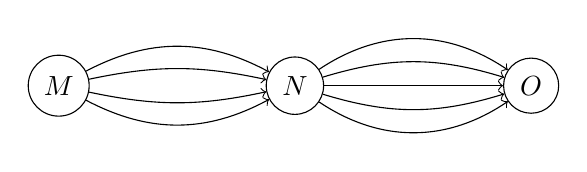
\begin{tikzpicture}[scale=1]
\node[draw,circle,minimum size=7mm](M)at(0,0){$M$};
\node[draw,circle,minimum size=7mm](N)at(3,0){$N$};
\node[draw,circle,minimum size=7mm](O)at(6,0){$O$};
\foreach \b in {28,12,-12,-28}\draw[->](M)to[bend left=\b](N);
\foreach \b in {34,17,0,-17,-34}\draw[->](N)to[bend left=\b](O);
\end{tikzpicture}}
Banyak cara perjalanan dari kota $M$ ke kota $O$ dan kembali ke kota $M$ melalui $N$ dengan ketentuan tidak melalui jalur yang sama adalah \ldots
\begin{pil}\item $180$ \item $240$ \item $260$ \item $160$ \item $120$\end{pil}
\end{soalbox}
\begin{pembox}
Dari gambar, terdapat 4 jalur $M\to N$ dan 5 jalur $N\to O$. Perjalanan berangkat $M\to O$: $4\cdot5=20$ cara. Saat pulang, jalur $O\to N$ tidak boleh sama dengan yang dipakai berangkat, tersisa $5-1=4$; jalur $N\to M$ juga tidak boleh sama, tersisa $4-1=3$. Total $20\cdot(4\cdot3)=240$.
\jw{(B) $240$}
\end{pembox}

\begin{soalbox}{9}
Titik berat dari segitiga $ABC$ adalah $Z$ dengan $A(1,0,2)$, $B(5,4,10)$, dan $C(0,-1,6)$. Koordinat $Z$ adalah \ldots
\begin{pil}\item $(2,-1,6)$ \item $(2,1,6)$ \item $(3,-1,6)$ \item $(3,2,6)$ \item $(6,1,3)$\end{pil}
\end{soalbox}
\begin{pembox}
Titik berat $Z=\left(\tfrac{x_A+x_B+x_C}{3},\tfrac{y_A+y_B+y_C}{3},\tfrac{z_A+z_B+z_C}{3}\right)=\left(\tfrac{1+5+0}{3},\tfrac{0+4-1}{3},\tfrac{2+10+6}{3}\right)=(2,1,6)$.
\jw{(B) $(2,1,6)$}
\end{pembox}

\begin{soalbox}{10}
Pada gambar berikut, $BD=CD$, panjang $AB=p$ satuan, dan $\angle BDA=x$. Panjang $BC$ adalah \ldots
\fig{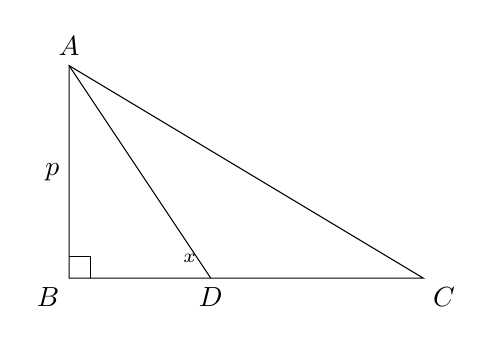
\begin{tikzpicture}[scale=0.9]
\coordinate(A)at(0,3);\coordinate(B)at(0,0);\coordinate(C)at(5,0);\coordinate(D)at(2,0);
\draw(A)--(B)--(C)--cycle;\draw(A)--(D);
\draw(0,0.3)--(0.3,0.3)--(0.3,0);
\node[above]at(A){$A$};\node[below left]at(B){$B$};\node[below right]at(C){$C$};\node[below]at(D){$D$};
\node[left]at($(A)!0.5!(B)$){$p$};
\node at(1.7,0.28){\scriptsize$x$};
\end{tikzpicture}}
\begin{pil}\item $\dfrac{p}{\tan x}$ \item $2p\tan x$ \item $p\tan x$ \item $\dfrac{2p}{\tan x}$ \item $2p\sin x$\end{pil}
\end{soalbox}
\begin{pembox}
Karena $BD=CD$, titik $D$ adalah titik tengah $BC$, sehingga $BC=2BD$. Pada segitiga siku-siku $ABD$, $\tan x=\tfrac{AB}{BD}=\tfrac{p}{BD}$, sehingga $BD=\tfrac{p}{\tan x}$. Maka $BC=2BD=\tfrac{2p}{\tan x}=2p\cot x$.
\jw{(D) $\dfrac{2p}{\tan x}$ (yaitu $2p\cot x$)}
\end{pembox}

\begin{soalbox}{11}
Vektor $\vec a$ dan $\vec b$ membentuk sudut tumpul $\alpha$, dengan $\sin\alpha=\tfrac{1}{\sqrt7}$. Jika $|\vec a|=\sqrt5$ dan $|\vec b|=\sqrt7$, maka $\vec a\cdot\vec b$ adalah \ldots
\begin{pil}\item $30$ \item $\sqrt{30}$ \item $-\sqrt{30}$ \item $-20$ \item $-30$\end{pil}
\end{soalbox}
\begin{pembox}
$\vec a\cdot\vec b=|\vec a||\vec b|\cos\alpha$. Karena $\alpha$ tumpul, $\cos\alpha=-\sqrt{1-\sin^2\alpha}=-\sqrt{1-\tfrac17}=-\sqrt{\tfrac67}$. Maka $\vec a\cdot\vec b=\sqrt5\cdot\sqrt7\cdot\left(-\sqrt{\tfrac67}\right)=-\sqrt{35\cdot\tfrac67}=-\sqrt{30}$.
\jw{(C) $-\sqrt{30}$}
\end{pembox}

\begin{soalbox}{12}
Hitung nilai limit $\displaystyle\lim_{x\to0}\dfrac{\tan x}{x^2\csc3x}=\ldots$
\begin{pil}\item $1$ \item $2$ \item $3$ \item $4$ \item $5$\end{pil}
\end{soalbox}
\begin{pembox}
Gunakan $\tan x\sim x$ dan $\sin3x\sim3x$ ketika $x\to0$. Karena $\csc3x=\tfrac{1}{\sin3x}$: $\dfrac{\tan x}{x^2\csc3x}=\dfrac{\tan x\sin3x}{x^2}$. Maka $\lim_{x\to0}\dfrac{\tan x\sin3x}{x^2}=\left(\lim\tfrac{\tan x}{x}\right)\left(\lim\tfrac{\sin3x}{x}\right)=1\cdot3=3$.
\jw{(C) $3$}
\end{pembox}

\begin{soalbox}{13}
Jika parabola $y=x^2$ memotong garis $y=x+2$ di titik $A$ dan $B$, maka panjang ruas garis $AB$ adalah \ldots
\begin{pil}\item $4$ \item $3$ \item $2$ \item $2\sqrt2$ \item $3\sqrt2$\end{pil}
\end{soalbox}
\begin{pembox}
Titik potong: $x^2=x+2\Rightarrow x^2-x-2=0\Rightarrow(x-2)(x+1)=0$, sehingga titiknya $(2,4)$ dan $(-1,1)$. Panjang $AB=\sqrt{(2-(-1))^2+(4-1)^2}=\sqrt{9+9}=3\sqrt2$.
\jw{(E) $3\sqrt2$}
\end{pembox}

\begin{soalbox}{14}
Nilai ${}^6P_3+{}^5P_2+{}^7P_4$ adalah \ldots
\begin{pil}\item $900$ \item $980$ \item $600$ \item $680$ \item $390$\end{pil}
\end{soalbox}
\begin{pembox}
${}^nP_r=\tfrac{n!}{(n-r)!}$. Maka ${}^6P_3=6\cdot5\cdot4=120$, ${}^5P_2=5\cdot4=20$, ${}^7P_4=7\cdot6\cdot5\cdot4=840$. Jumlahnya $120+20+840=980$.
\jw{(B) $980$}
\end{pembox}

\begin{soalbox}{15}
Diketahui suatu deret geometri tak hingga dengan suku awal $a$ dan rasio $r$. Jika jumlah suku awal dan rasionya sama dengan 6 dan jumlah semua sukunya sama dengan 5, maka $\dfrac{a}{r}$ adalah \ldots
\begin{pil}\item $-20$ \item $25$ \item $\dfrac56$ \item $-\dfrac{1}{25}$ \item $-25$\end{pil}
\end{soalbox}
\begin{pembox}
$S_\infty=\dfrac{a}{1-r}=5$ dan $a+r=6$. Dari $a=5(1-r)=5-5r$, substitusi: $5-5r+r=6\Rightarrow-4r=1\Rightarrow r=-\tfrac14$. Maka $a=6-r=6+\tfrac14=\tfrac{25}{4}$, sehingga $\dfrac{a}{r}=\dfrac{25/4}{-1/4}=-25$.
\jw{(E) $-25$}
\end{pembox}

\medskip\hrule\medskip
{\noindent\bfseries Kunci Jawaban Bagian IV:}\\
1 (lihat catatan; C jika $\tan c=\tfrac15$), 2 D, 3 B, 4 (tidak ada opsi), 5 C, 6 A, 7 D, 8 B, 9 B, 10 D, 11 C, 12 C, 13 E, 14 B, 15 E.

\medskip\hrule\medskip
{\noindent\small\itshape Tanda * atau ``tidak ada opsi'' menunjukkan nomor dengan catatan redaksi karena hasil pindai/opsi pada naskah sumber tidak sepenuhnya konsisten dengan perhitungan logis.}

\end{document}
